%%%%%%%%%%%%%
\chapter{Ergebnisdiskussion}
\label{ch:Results}
%%%%%%%%%%%%%
Zur Bewertung der Konzepte werden die in Kapitel \ref{ch:evaluation} beschriebenen Daten zunächst interpretiert. Die Ergebnisse der Interpretation werden anschließend kritisch betrachtet und, basierend auf der Ergebnisinterpretation, ein Ausblick der nächsten Schritte, für die Umsetzung des \emph{TMA} beschrieben. 


\section{Ergebnisinterpretation}
Die Ergebnisinterpretation erfolgt auf den, in Kapitel \ref{ch:evaluation}, aufgestellten Hypothesen. Ziel der Ergebnisinterpretation ist darzulegen, dass ein Modellierungsansatz nach dem Konfigurationsprinzip für den späteren Anwender verständlicher ist. Als Baseline dient hierfür das \emph{movisensXS}-System, welches ein Konstruktionsprinzip verfolgt. Dieser Ansatz bietet im Vergleich sehr viel Flexibilität in der Gestaltung einer Therapie. Die Ergebnisse werden kategorisiert betrachtet. Gegenübergestellt werden jeweils, wie bisher, das Konstruktionsprinzip und Konfigurationsprinzip, sowie der Einsatz von Sprüngen und die Verwendung von Sichtbarkeitsregeln. Die Betrachtung der Ergebnisse wird gemäß der zuvor verwendeten Reihenfolge erfolgen. Abschließend werden die Ergebnisse zusammengefasst dargestellt.


\subsection{Konfigurationsprinzip und Konstruktionsprinzip}
Eine erste Betrachtung der Ergebnisse, deutet darauf hin, dass die Nutzer die Umsetzung und Verwendung des Konfigurationsprinzips besser bewerteten als das Konstruktionsprinzip. Wie in Abbildung \ref{antwortendurchsch11} und Abbildung \ref{antwortendurchsch22} zu sehen ist, haben die Probanden den \emph{TherapyBuilder}-Prototyp im Schnitt besser bewertet als das angepasste \emph{movisensXS}-System. Diese Ergebnisse wurden den Zwischenfragebögen entnommen und zeigen eine erste Tendenz auf. 

Auch die Ergebnisse der Abschlussfragerunde geben einen ersten Hinweis auf die Bewertung der Verständlichkeit und Übersicht beider Prinzipien. Insgesamt konnten die Probanden in der Abschlussfragerunde achtundzwanzig Punkte nennen (vgl. Abbildung \ref{konstrabsch} und \ref{konfigabsch}), die ihnen am Konstruktionsprinzip gut gefallen haben und die sie besonders hilfreich empfanden. Zum Konfigurationsprinzip äußerten sie hierzu hingegen neununddreißig Punkte. Die Probanden konnten somit bezüglich des Konfigurationsprinzips insgesamt mehr Punkte äußern, die ihnen an dieser Umsetzung gut gefallen haben und besonders hilfreich empfunden wurden. Betrachtet man diese jedoch im Einzelnen, wurden Konstruktionsprinzip mehr Punkte dahingehend geäußert, was den Probanden gut gefallen hat. Hinsichtlich der Nachfrage, was den Probanden an der jeweiligen Umsetzung nicht gefallen hat und was sie vermisst haben, schnitt auch hier das Konfigurationsprinzip besser ab. Im Vergleich zum Konstruktionsprinzip fielen den Probanden neunzehn Punkte ein. Das sind dreizehn Punkte weniger als die Probanden zum Konstruktionsprinzip äußerten. Zwar gibt es insgesamt mehr positive Anmerkungen bezüglich des Konfigurationsprinzip, allerdings wurden gegenüber dem Konstruktionsansatz mehr Punkte genannt, die den Probanden an diesem Ansatz besonders gut gefallen haben. Welche Punkte das sind und wie sich diese mit den Ergebnissen und aufgestellten Hypothesen verbinden lassen, wird im Verlauf dieses Kapitels betrachtet.


\begin{figure}
   \begin{minipage}[b]{.49\linewidth} % [b] => Ausrichtung an \caption
      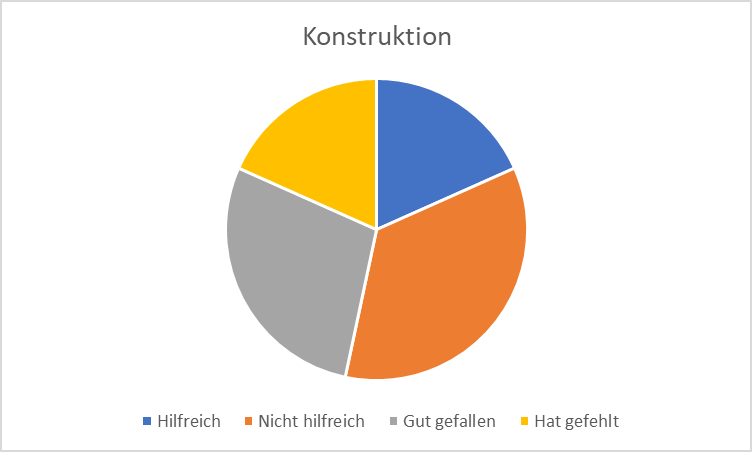
\includegraphics[width=\linewidth]{pictures/diagramme/aussagenkonstr}
      \caption{Zu sehen ist die Anzahl der genannten Punkte der Abschlussfragerunde. Die Probanden nannten achtundzwanzig Punkte auf die Frage was ihnen am Konstruktionsprinzip gut gefällt und sie als hilfreich empfinden}
      \label{konstrabsch}
   \end{minipage}
   \hspace{.01\linewidth}% Abstand zwischen Bilder
   \begin{minipage}[b]{.49\linewidth} % [b] => Ausrichtung an \caption
      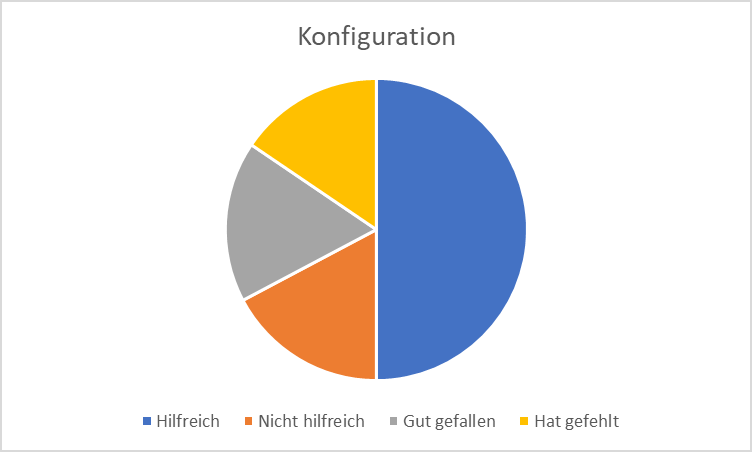
\includegraphics[width=\linewidth]{pictures/diagramme/aussagenkonfig}
      \caption{Im Vergleich äußerten die Probanden deutlich mehr Punkte, die sie am umgesetzten Konfigurationsprinzip als hilfreich empfinden. Allerdings konnten sie auch weniger Aussagen darüber treffen, was ihnen besonders gut gefallen hat}
      \label{konfigabsch}
   \end{minipage}
\end{figure}



\paragraph{Verständlichkeit der Triggereinstellungen}
Die Ergebnisse der Zwischenfragebögen zeigen eine Tendenz, dass im Vergleich das Kontruktionsprinzip für Anwender verständlicher ist. Die Freitexte der Zwischenfragebögen und Abschlussfragerunde deuten hingegen darauf hin, dass zwar viele Einstellungsmöglichkeiten geboten werden ohne mit diesen zu erschlagen und gefühlt weniger Einstellungsschritte und notwendig sind. Der Fluss vom Klicken wirkt klarer und konsistenter. Allerdings äußerten mehrere Probanden, dass die Einstellungen der Trigger zunächst irritierten. Betrachtet man die Ergebnisse der Abschlussfragerunde bestätigt sich letztere Aussage. Die Hälfte der Probanden wünschen sich eine Anleitung oder Tooltips zum besseren Verständnis der Triggereinstellungen.

Zwar wurde das \emph{movisensXS}-System im Zwischenfragebogen hinsichtlich der Triggereinstellungen schlechter bewertet. Dennoch kann das verwendete Konstruktionsprinzip mit seiner flexiblen Gestaltungsmöglichkeit aufwarten. Die Einstellungen der Trigger werden bei wachsender Komplexität unübersichtlicher. Aber insbesondere die vielen Einstellungsmöglichkeiten via Drag and Drop durch das Baukastenprinzip, und die Flexibilität in der Anordnung und Gestaltung, sind generell besser nachvollziehbar. Nicht nur das Baukastenprinzip und die einhergehende Drag and Drop Funktion tragen dazu bei, sondernm auch die Trennung verschiedener Elemente anhand ihrer Funktion. 

Insgesamt ist zwar eine Tendenz gegeben, dass das Konstruktionsprinzip leichter verständlich ist, allerdings benötigt dieses zusätzlich Anleitungen und Tooltips um diese zu verbessern. Auch wenn das Konstruktionsprinzip tendenziell schlechter abschneidet, so ist gerade das zusammenbauen der Triggereinstellungen für die Nutzer interessant und das Prinzip an sich leicht nachvollziehbar. Allerdings kann hier auch die flexible Anordnung zu einer geringeren Übersicht beitragen. Hier könnte eine automatische Anordnungsfunktion, oder Anordnungshilfe zur besseren Übersicht beitragen.


\paragraph{Verständlichkeit der Triggerdarstellung}
Auch hier lässt sich in Abbildung \ref{antwortendurchsch1} eine leichte Tendenz erkennen, dass die Triggerdarstellung im Konfigurationsprinzip verständlicher ist. Der Unterschied zwischen dem Konstruktionsprinzip und Konfigurationsprinzip ist hier allerdings relativ gering. Insbesondere die zeitliche Übersicht und das Zusammenbringen der Einstellungen und dem Ablauf empfanden die Probanden als positiv. Allerdings kristallisiert sich heraus, dass die Farben zwar zur Übersicht beitragen. Nur eine Erklärung dessen fehlt zum besseren Verständnis. Generell wurde die Darstellung zwar als übersichtlich beschrieben, aber die Verständlichkeit leidet unter den fehlenden Erläuterungen zu den angebotenen Farben, Symbolen und anderen Darstellungsformen. 

Das Konstruktionsprinzip hingegen wird zwar in der Darstellung schnell unübersichtlich, aber besonders die Farben der einzelnen Bausteine helfen beim Orientieren. Außerdem beinhaltet die Darstellung mehr Informationen auf einem Blick. Besonders die farbliche Kodierung der Blöcke wird von den Probanden positiv hervorgehoben. 

Zwar schneidet das Konfigurationsprinzip besser ab, allerdings nur geringfügig. das Konstruktionsprinzip hebt sich besonders durch die farbliche Kodierung hervor. Diese Eigenschaft kann sich das Konfigurationsprinzip zu eigen machen. Eine durchdachte farbliche Kodierung der Trigger in Kombination mit entsprechenden Symbolen und einer ausführlichen Legende mit Erklärungen, können erheblich zu einer verständlicheren Darstellung der Trigger beitragen. Auch das hinterlegen von Informationen über die Triggereinstellungen, in Form von Tooltips an den zeitlich dargestellten Elementen, können sich positiv auf das Konfigurationsprinzip auswirken. Auch hier kann das Konstruktionsprinzip von einer strikteren Anordnungsvorgabe profitieren. 

\paragraph{Übersichtlichkeit der Konversationen}
Betrachtet man die erhobenen Daten hinsichtlich der Übersichtlichkeit innerhalb der verschiedenen Konzepte, so lässt sich auch hier eine Tendenz erkennen. Wie in Abbildung \ref{antwortendurchsch22} zu sehen, schneidet das Konfigurationsprinzip des \emph{TherapyBuilders} besser in der Fragebogenauswertung ab als das Konstruktiosnprinzip. Die Tendenz zeigt, dass die Listendarstellung aller Konversationen innerhalb der Darstellung des Konfigurationsprinzip, übersichtlicher gestaltet ist, als die freie Anordnung innerhalb des Konstruktionsprinzips des \emph{movisensXS}. Die Ergebnisse der Abschlussfragerunde bekräftigen die Ergebnisse des Fragebogens. Besonders die Listendarstellung und die hierfür angebotene Suchmöglichkeit nach einzelnen Konversationen werden als positive Punkte angebracht. Diese wird im Konstruktionsprinzip hingegen vermisst. Will der Nutzer eine Konversation und dessen Triggereinstellungen betrachten, muss diese erst im Baum gesucht werden. 

Triggereinstellungen einer Konversation einzusehen, gestaltet sich im Konfigurationsprinzip tendenziell leichter. Eine Suchfunktion könnte das Konstruktionsprinzip in diesem Punkt verbessern.


\paragraph{Übersichtlichkeit der zeitlichen Darstellung der Konversationen}
Abbildung \ref{antwortendurchsch22} verdeutlicht die unterschiedliche Bewertung beider Systeme hinsichtlich ihrer zeitlichen Darstellung der Konversationen. Es zeichnet sich eine deutliche Tendenz ab, dass diese innerhalb des Konfigurationsprinzips eine bessere Übersicht über die zeitliche Steuerung der Konversationen besteht. Die Ergebnisse der Freitexte, sowie der Abschlussfragerunde, untermauern das Ergebnis. So ist der zeitliche Ablauf und die Darstellung im Zeitstrahl übersichtlich, leicht nachvollziehbar. Außerdem lässt sich die spätere Belastung des Patienten einsehen. Alle Probanden äußerten sich positiv über diese Art der Darstellung. Ein Proband vermisst allerdings Funktionen bei dieser Darstellung. So wünscht sich dieser eine Möglichkeit auf einzelne Elemente zu klicken und eine Funktion damit auszulösen. Hingegen wurde das Konstruktionsprinzip in diesem Punkt ausschließlich kritisiert. Der zeitliche Ablauf der Konversationen ist schwer zu überblicken. 

Das Konfigurationsprinzip kann leicht um den Punkt der klickbaren Elemente und einer dahinter versteckten Funktion, wie beispielsweise das Aufrufen der Trigger-Einstellungen, erweitert werden. Um das Konstruktionsprinzip in diesem Punkt zu verbessern, könnte eine stärkere Vorgabe für die Strukturierung und Anordnung der Elemente auf dem entsprechenden Arbeitsblatt hilfreich sein. So könnte auch eine zeitliche Abfolge der Konversationen dargestellt werden.


\paragraph{Verständlichkeit der Triggerkonfiguration}
Hinsichtlich der Konfigurierung der Trigger wurde der \emph{TherapyBuilder}-Prototyp schlechter bewertet als der \emph{movisensXS}-Prototyp. Es ist eine Tendenz erkennbar, die aufzeigt, dass das Konstruktionsprinzip hinsichtlich der Triggerkonfiguration verständlicher ist. Die Betrachtung der Freitext-Aussagen sowie der Abschlussfragerunde geben Hinweise, in welchen Punkten sich das Konstruktionsprinzip hervorhebt. So ist insbesondere die Anordnung der Bausteine leicht verständlich. Die Drag and Drop Funktion erleichtert diese außerdem. Die einhergehende Flexibilität der Anordnung, sowie die farbliche Kodierung der Bausteine fallen positiv auf und tragen der Verständlichkeit bei. Diese wird beim Konfigurationsprinzip vermisst. So sind die Einstellungen der Konditionen nicht ganz klar. Außerdem lässt sich die Bearbeitungsfunktion der Trigger schwer finden. 

Um die Konfiguration der Trigger des Konfigurationsprinzip verständlicher zu gestalten, benötigt es zunächst einen besseren Zugang zu den Einstellungen. Außerdem sollten die Funktionen und Einstellungen erneut überarbeitet werden. Hier könnte eine strengere Form des Konstruktionsprinzips verwendet werden um die Einstellungsmöglichkeiten flexibel und verständlich zu gestalten. Möglich wäre eine Vorgabe von kleinen Bausteinen, die beliebig angeordnet, farblich kodiert und eingestellt werden können, sich allerdings nur auf eine Konversation bezieht, statt, wie im Konstruktionsprinzip, auf beliebig viele. Diese Form könnte die Übersichtlichkeit des Konfigurationsprinzip beibehalten.


\paragraph{Verständlichkeit von Abhängigkeiten zwischen Konversationen und Konversationsverzweigungen}
Die Abhängigkeiten zwischen Konversationen ist im Vergleich zum 
Die Grafiken \ref{antwortendurchsch11} und \ref{antwortendurchsch22} verdeutlichen eine positive Tendenz hinsichtlich der Verständlichkeit von Konversationsverzweigungen und Abhängigkeiten zwischen Konversationen im \emph{TherapyBuilder}. Das dort eingesetzte Konfigurationsprinzip wird in diesem Punkt allerdings kaum in den Freitext-Aussagen sowie der Abschlussfragerunde erwähnt. Nur zwei Probanden äußern, dass die Darstellung der Abhängigkeiten gut einsehbar sind. Der \emph{movisensXS}-Prototyp wird generell als weniger übersichtlich und verständlich bezüglich des zeitlichen Verlaufs beschrieben. Allerdings geht auch hier kein Proband genauer auf die Abhängigkeiten zwischen Konversationen ein. 

Generell könnte das Konstruktionsprinzip des \emph{TherapyBuilder} auch in diesem Punkt durch eine verständliche und ausführliche Legende, sowie Tooltips mit entsprechenden Informationen, die Verständlichkeit der Abhängigkeiten verbessern. Das Konstruktionsprinzip könnte auch hier von einer strikteren Anordnungsvorgabe profitieren. 

\paragraph{Übersichtlichkeit der Therapie}
Insgesamt zeichnet sich eine Tendenz ab, die aufzeigt, dass eine Therapie im Konfigurationsprinzip übersichtlicher dargestellt ist als im Konstruktionsprinzip. Dies wird zunächst durch die Auswertung der Fragebögen (vgl. Abbildung \ref{antwortendurchsch22} angedeutet. Die Freitext-Aussagen und Ergebnisse der Abschlussfragerunde ergeben, dass die Umsetzung des Konstruktionsprinzips die Übersichtlichkeit über die gesamte Therapie vermissen lässt. Im Gegensatz zum Konfigurationsprinzip kann hier nur schwer die Belastung des Patienten und die zeitliche Abfolge nachvollzogen werden. Diese könnte innerhalb des Konstruktionsprinzips durch bereits genannte, strikte Anordnungsregeln, verbessert werden. Zur Verbesserung dieser sollte, die mögliche Darstellung der zeitlichen Abfolge, wie auch der Abhängigkeiten zwischen verschiedenen Konversationen, berücksichtigt werden.



\subsection{Sprünge und Sichtbarkeitsregeln}
Vergleicht man insgesamt die Ergebnisse der Prototypen hinsichtlich der Verwendung von Sprüngen und Sichtbarkeitsregeln, so schneidet auf den ersten Blick der \emph{TherapyBuilder}-Prototyp ab. Nachfolgend werden, anhand der zuvor aufgestellten Hypothesen, die verschiedenen Konzepte genauer betrachtet und bewertet. Verglichen werden diese Konzepte hinsichtlich ihres Einflusses auf die Verständlichkeit und Übersichtlichkeit der einer Chatbot-Konversation.


\begin{figure}
   \begin{minipage}[b]{.49\linewidth} % [b] => Ausrichtung an \caption
      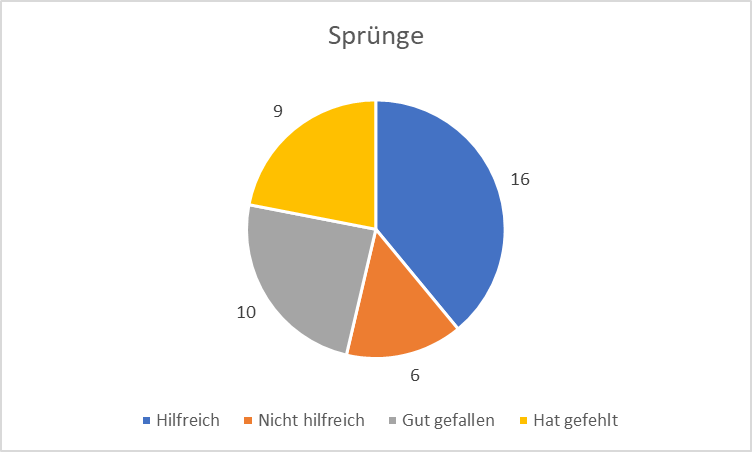
\includegraphics[width=\linewidth]{pictures/diagramme/aussagenspr}
      \caption{Wasser}
   \end{minipage}
   \hspace{.01\linewidth}% Abstand zwischen Bilder
   \begin{minipage}[b]{.49\linewidth} % [b] => Ausrichtung an \caption
      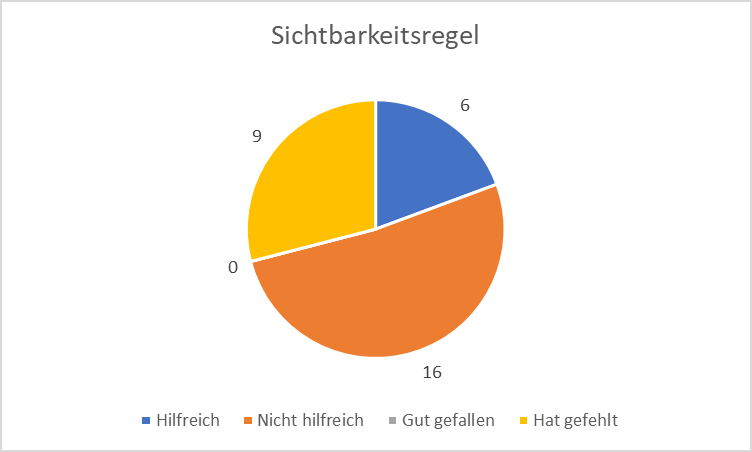
\includegraphics[width=\linewidth]{pictures/diagramme/aussagensichtb}
      \caption{Land}
   \end{minipage}
\end{figure}

\paragraph{Verständlichkeit der Konversationsdarstellung}

\paragraph{Verständlichkeit der Konversationseinstellungen}

\paragraph{Übersichtlichkeit des Konversationsverlaufs}

\paragraph{Übersichtlichkeit der Antwortoptionen innerhalb des Konversationsverlaufs}

\paragraph{Verständlichkeit der Verzweigungen innerhalb des Konversationsverlaufs}

\paragraph{Übersichtlichkeit der Werkzeugpalette zur Konversationserstellung}




\subsection{Zusammenfassung}

\section{Kritische Reflexion}

\begin{figure}[h]
\centering
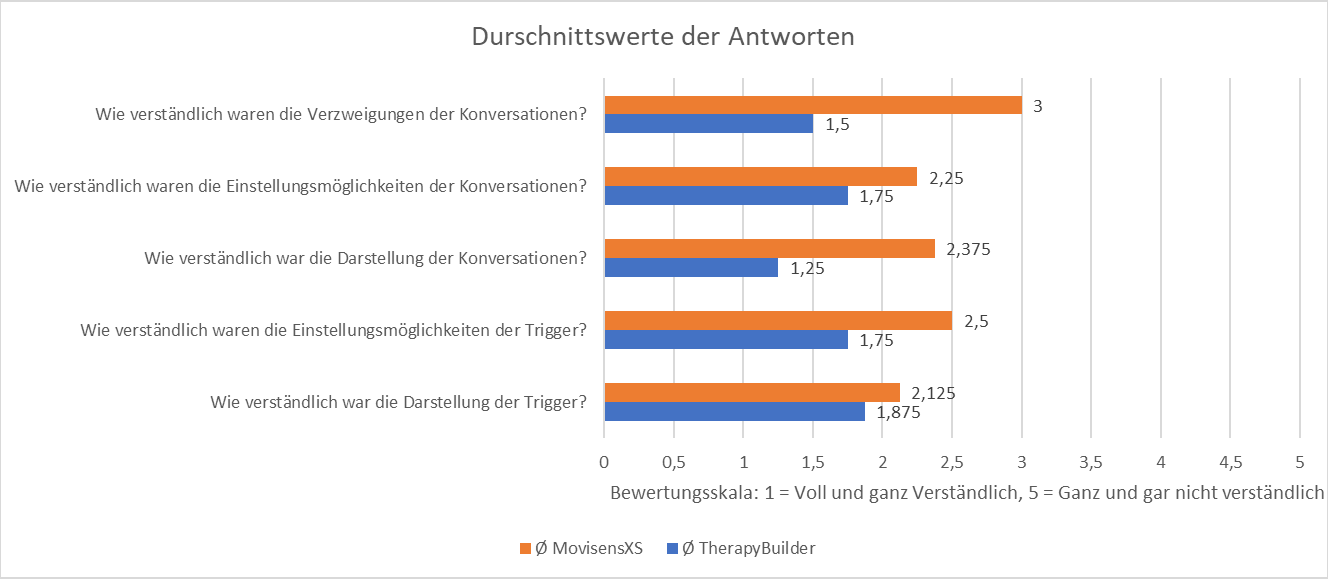
\includegraphics[width=1\textwidth]{pictures/diagramme/antwortendurchsch1}
\caption{Architektur des \emph{konfiguration}}
\label{antwortendurchsch11}
\end{figure}

\begin{figure}[h]
\centering
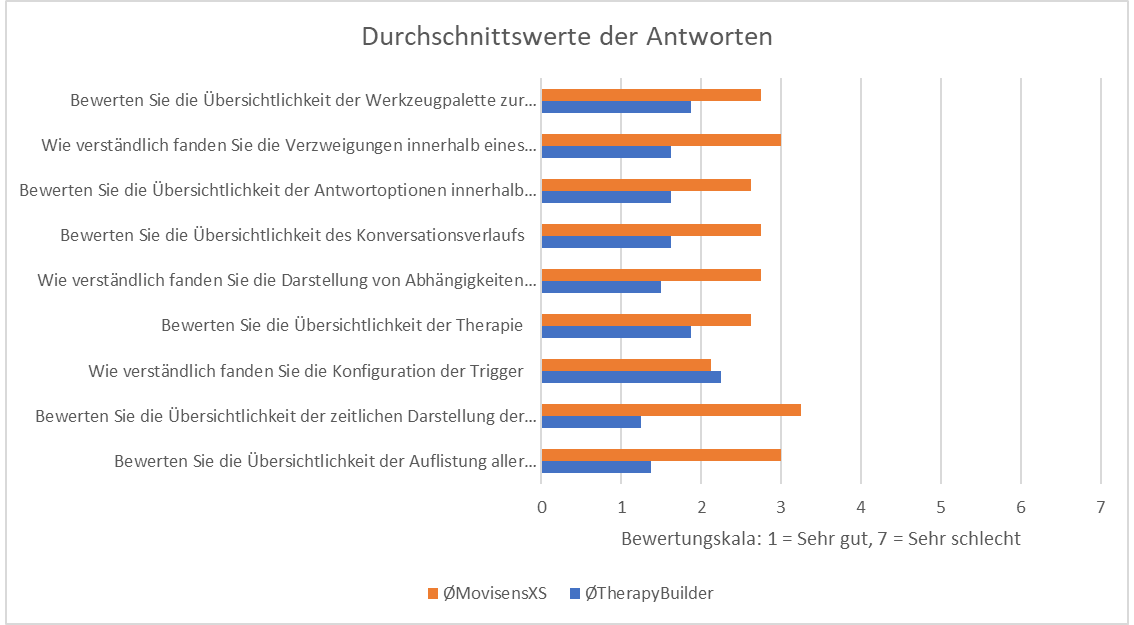
\includegraphics[width=1\textwidth]{pictures/diagramme/antwortendurchsch2}
\caption{Architektur des \emph{konfiguration}}
\label{antwortendurchsch22}
\end{figure}

